\documentclass{article}
\usepackage{graphicx}
\usepackage[utf8]{inputenc}
\usepackage{textcomp}
\usepackage[spanish]{babel}
\usepackage{xcolor}
\usepackage{listings}


\definecolor{comment}{RGB}{127, 127, 127}

\lstdefinestyle{pseudo}{
    basicstyle=\ttfamily\footnotesize,
    breaklines=true,
    keepspaces=true,
    frame=single,
    captionpos=b,
    rulecolor=\color{gray},
    moredelim=[s][\color{comment}\bfseries]{\#}{.}
}

\begin{document}

\begin{titlepage}
    \centering
    \vspace*{1cm}
    
    % Logo
    
\includegraphics[width=0.2\textwidth]{imagenes/logo.png}\par\vspace{0.5cm}
    
    % Título
    {\scshape\Large Teoría de Algoritmos (TB024/75.29)\par}
    \vspace{1.5cm}
    {\LARGE Trabajo Práctico N° 2\par}
    {\huge\bfseries Redes de flujo, Clases de Complejidad y Fuerza Bruta\par}
    \vspace{2cm}
    
    % Autor
    {\Large Grupo 3SAT \par}
    \vfill
    
    % Profesor
    Profesor:\par
    Ing. Victor Podberezky\par
    \vfill
    
    % Fecha
    {\large \today\par}
\end{titlepage}

\tableofcontents
\newpage

\section{Introducción}

    El estudio avanzado de algoritmos permite no solo resolver problemas de manera eficiente, sino también comprender las limitaciones intrínsecas de la computación y la estructura subyacente de problemas complejos de optimización. Mientras que las técnicas de diseño clásicas proporcionan herramientas para construir soluciones, el análisis de flujos en redes y la clasificación de problemas según su complejidad permiten determinar la viabilidad de dichas soluciones en entornos reales. 
    
    En el presente informe, se profundizará en el estudio de tres ejes fundamentales de la algoritmia moderna: la modelización mediante redes de flujo, la implementación de estrategias de búsqueda exhaustiva y el marco teórico de las clases de complejidad.En la primera parte de este trabajo, se abordará la teoría de Redes de Flujo, una herramienta esencial para resolver problemas de transporte, logística y asignación de recursos. Se analizará cómo modelar un sistema de capacidades para determinar el flujo máximo posible entre nodos, aplicando conceptos como el teorema de Max-Flow Min-Cut. 
    
    Posteriormente, se explorará la técnica de Fuerza Bruta, evaluando su utilidad como punto de partida para la resolución de problemas combinatorios y discutiendo el costo computacional que implica la exploración completa del espacio de soluciones. 
    
    Finalmente, se presentará un análisis sobre las Clases de Complejidad, estableciendo las distinciones fundamentales entre problemas de las clases \textit{P}, \textit{NP} y \textit{NP-completos}. Este apartado permitirá comprender la frontera entre lo tratable y lo intratable, brindando al futuro ingeniero los criterios necesarios para identificar cuándo un problema exige una solución heurística o aproximada frente a la imposibilidad de hallar una solución exacta en tiempo polinomial.

\section{Desarrollo del trabajo}

    \subsection{La separación del Dojo}

        Las redes de flujo permiten modelar una gran variedad de problemas. Es posible representar cada arista dirigida como un conducto con capacidad limitada para transportar un fluido, y cada vértice como una intersección de dichos conductos. En consecuencia, por la ley de conservación, la cantidad de fluido que sale de cada intersección debe ser igual a la que ingresa. Gracias a esta relación de equilibrio, es posible identificar características que permiten resolver problemas complejos mediante una reducción polinomial a una red de flujo.

        El conocimiento sobre el comportamiento del flujo, el valor máximo que puede alcanzar la red y la identificación del ``cuello de botella'', determinado por el corte que minimiza la capacidad entre la fuente y el sumidero, es lo que permite adaptar este modelo a problemas que, a simple vista, no parecen tener una estructura de red. De esta forma, se logran soluciones algorítmicas eficientes para desafíos de optimización y particionamiento.

        \subsubsection{Explicación del problema}

            Un dojo tiene ``n'' miembros, dos de ellos son profesores, cada uno de los miembros del dojo se relacionó al menos una vez con alguno de los profesores. Dado un grupo de relaciones $R_{A}$, cuyos elementos son tuplas del tipo $[(m_{i}, m_{j}), r_{ij}]$ donde $m_{i}$ y $m_{j}$ son miembros del dojo tal que $m_{i} \ne m_{j}$ y $r_{ij}$ es un entero positivo representativo de las veces que se relacionó el miembro $m_{i}$ con $m_{j}$, se busca dividir a los miembros del dojo entre los dos profesores de forma que la cantidad de veces que se relacionaron dos miembros de un grupo sea la máxima posible. 

            \textbf{Supuestos del problema:} Se supone que cada miembro del dojo se relacionó al menos una vez con alguno de los profesores, y que en el grupo de relaciones no pueden haber relaciones negativas. Además se supone que el primer profesor $p_1$ tiene número de miembro 1 y el profesor $p_2$ tiene numero de miembro ``n''.

        \subsubsection{Propuesta de solución por red de flujos}

            Dado el grupo de relaciones $R_A$ y un grafo vacío $G$ se crea un vertice por cada miembro $m_i$ presente en $R_A$. Por cada relación $(m_i, m_j)$ se crea una arista dirigida $m_i \rightarrow m_j$ de tal forma que $i<j$, con capacidad $r_{ij}$. La restricción ``$i<j$'' genera que $p_1$ funcione como fuente (nodo $s$, del inglés \textit{source}) y que $p_2$ funcione como sumidero de la red (nodo $t$, \textit{terminal}), y que las aristas fluyan en el sentido $s \rightarrow t$.

             \begin{figure}[h]
                \centering
                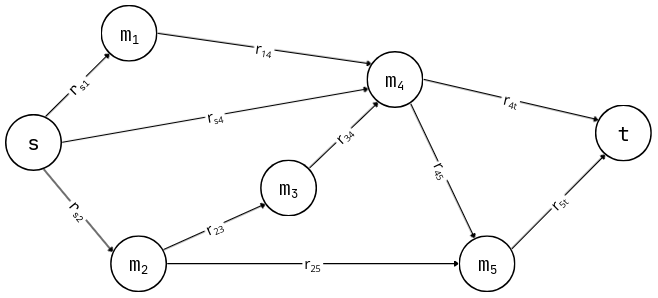
\includegraphics[width=0.8\textwidth]{imagenes/red-relacion.png}
                \caption{Ejemplo de red de flujo de relaciones}\label{red-relaciones}
             \end{figure}

            Bajo la premisa de buscar que los grupos mantengan la máxima relación entre sus miembros, se busca la partición de esta red que minimice la suma de los pesos de las relaciones que se pierden en la separación.

            Para lograrlo, en un primer paso de solución se calcula el flujo máximo de la red a través del Algoritmo de Edmonds-Karp. Por teorema fundamental de flujo se conoce que el valor de flujo máximo es igual a la capacidad de corte mínimo, donde el corte mínimo $(S, T)$ es una partición de los nodos tal que $s \in S$ y $t \in T$. Estos subconjuntos $S$ y $T$ contienen aquellos nodos tal que en $S$ se encuentran todos los nodos \textit{alcanzables} por $s$ en el grafo residual, es decir todos los nodos a los que se pueden llegar usando aristas de capacidad diferente de 0, y en T se encuentran los nodos que cumplen $T=G-\{S\}$.

            \begin{figure}[h]
                \centering
                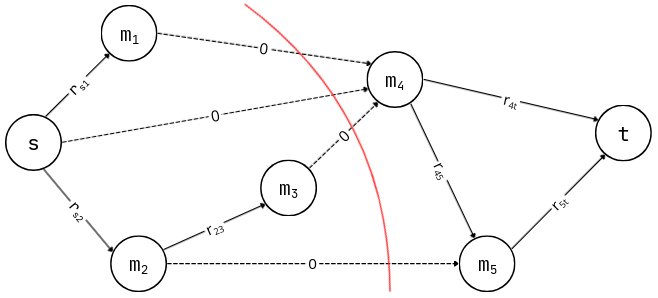
\includegraphics[width=0.8\textwidth]{imagenes/mincut.png}
                \caption{Corte mínimo de la red de relaciones}\label{mincut}
            \end{figure}

            Una vez obtenidos los dos subconjuntos de $G$ se comparan los tamaños de ambos para determinar cual de los dos grupos es el mayor y así poder retornar dicho grupo. Una posible implementación del código solución de esta propuesta puede ser el siguiente:

            \begin{lstlisting}[style=pseudo,caption={Pseudocódigo de la solución}]
function definirNuevoRepresentante(miembros V, relaciones R, profesores P1, P2):
    G = Grafo new;
    for(relacion r = ((u, v), i) in R):
        if(u not in G.V):
            G.V.add(u);
        if(v not in G.V):
            G.V.add(v);
        G.E.add((u,v), i);
    
    s, t = P1, P2;
    G', _ = FlujoMaximo(G, s, t); # Esto genera el grafo residual.
    
    miembros_p1 = {s};
    cola = [s]
    visitados = {s}

    while(cola not empty):
        u = cola.pop(0)
        for(vecino v de u en G'):
            if(v not in visitados && G'.capacidad(u,v) > 0):
                visitados.add(v)
                miembros_p1.add(v)
                cola.add(v)
    
    miembros_p2 = G.V.notIn(miembros_p1)

    if(|miembros_p1| > |miembros_p2|):
        return P1;
    else if(|miembros_p1| < |miembros_p2|):
        return P2;
    else:
        return "Ambos profesores se dividen la misma cantidad de alumnos";
            \end{lstlisting}

            Donde la función \texttt{FlujoMaximo()} está determinada por el siguiente Pseudocódigo:

            \begin{lstlisting}[style=pseudo,caption={Pseudocódigo de FlujoMaximo}]
function FlujoMaximo(Grafo G, fuente s, sumidero t):
    for each(eje e in G):
        e.flujo = 0
    
    G_res = construirGrafoResidual(G)
    flujo_total = 0
    
    while(existeCamino(G_res, s, t)):
        P = G_res.shortestPath(s, t)
        
        w = P.getBottleneck()
        
        G.aplicarAumento(P, w)
        G_res.actualizarCapacidades(P, w)
        
        flujo_total += w
        
    return G_res, flujo_total
            \end{lstlisting}

        \subsubsection{Análisis de la solución}



\subsection{El despacho de los productos}

\subsubsection{Explicación del problema}

\subsection{Los centros de atención}

\section{Conclusión}

A partir de este trabajo de investigación y de la puesta en práctica de los conocimientos obtenidos en esta etapa avanzada de la Teoría de Algoritmos, se ha logrado profundizar en el análisis de problemas de optimización de alta complejidad. El estudio de las Redes de Flujo permitió comprender la modelización de sistemas con restricciones de capacidad, mientras que el abordaje de la Fuerza Bruta y las Clases de Complejidad brindó una perspectiva integral sobre los límites de la eficiencia computacional y la distinción entre problemas tratables e intratables.

Asimismo, se enriqueció la labor realizada mediante una investigación exhaustiva que integró tanto el material bibliográfico de la cátedra como el análisis de publicaciones técnicas y recursos académicos complementarios. Esta base teórica fue fundamental para entender no solo el funcionamiento de los algoritmos, sino también las implicancias de las reducciones entre problemas y la jerarquía de complejidad que rige a la informática moderna.

Finalmente, la implementación en el lenguaje Python de las soluciones propuestas para redes de flujo y algoritmos de búsqueda exhaustiva resultó clave para validar los modelos teóricos. Este proceso permitió observar el comportamiento real de los algoritmos frente a diferentes volúmenes de datos y casos de prueba, consolidando la transición entre el diseño conceptual y la aplicación práctica de soluciones óptimas en entornos de ingeniería.

\section{Referencias}



\end{document}
